\subsection{Circunferencia y Círculo}
Dado un punto $O$, y una distancia $r$, la circunferencia está definida por el conjunto (infinito) de todos los puntos en el plano que están a una distancia $r$ de $O$. Un círculo corresponde a la circunferencia junto con la región inscrita dentro de ella.\\

\subsubsection{Ángulos de una Circunferencia}
\textit{Ángulo de Centro:} Vértice en el centro, sus lados son dos radios.\\
\textit{Ángulo Interior:} Vértice dentro de la circunferencia (no en ella!), sus lados son dos cuerdas.\\
\textit{Ángulo Exterior:} Vértice fuera de la circunferencia, sus lados son dos secantes, una secante y una tangente, o dos tangentes.\\
\textit{Angulo Inscrito:} Vértice en la circunferencia, los lados son dos secantes o cuerdas.\\
\textit{Ángulo semiinscrito:} Vértice en la circunferencia, un lado secante y otro tangente.\\

\subsubsection{Teoremas de Ángulos}
Unidades: $360^{\circ} = \SI{2\pi}{\radian}$\\

Con $\angle ACB$ inscrito y $\angle AOB$ de centro,
$\measuredangle ACB = \frac{\measuredangle AOB}{2}$.\\

Análogamente, con $\angle ABC$ semiinscrito (tangente), y $\angle BOC$ de centro, $\measuredangle ABC = \frac{\measuredangle BOC}{2}$.\\

La medida de un \textbf{ángulo interior} es igual a la semisuma de las medidas angulares (de centro) de los arcos formados por dicho ángulo:
\begin{equation*}
    \measuredangle APB = \frac{m(\stackrel\frown{AB}) + m(\stackrel\frown{CD})}{2}
\end{equation*}
Con $\angle APB$ interior, y $\stackrel\frown{AB}$ y $\stackrel\frown{CD}$ arcos formados por el.\\

De la misma forma, la medida de un \textbf{ángulo exterior} es igual a la semidiferencia de los ángulos de centro formados por el ángulo. (mayor primero)
\begin{equation*}
    \measuredangle APB = \frac{m(\stackrel\frown{AB}) - m(\stackrel\frown{CD})}{2}
\end{equation*}

\subsubsection{Teoremas de Trazos}
\textbf{Teorema de las Cuerdas}\\

\begin{center}
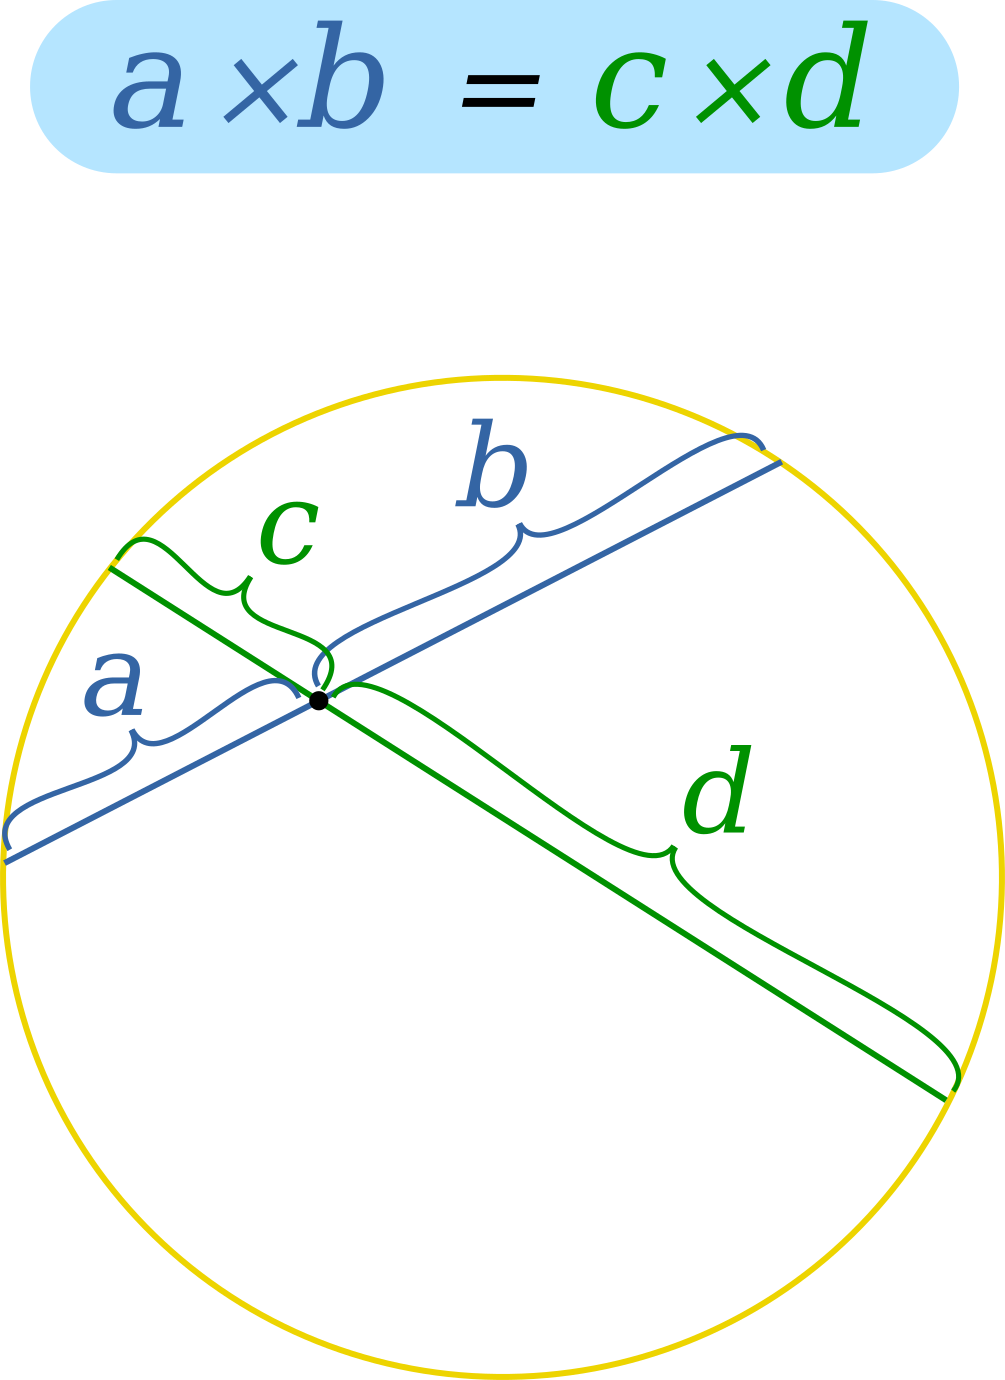
\includegraphics[width=0.5\columnwidth]{teoremacuerdas}
\end{center}
\textbf{Teorema de las Secantes}\\
\begin{center}
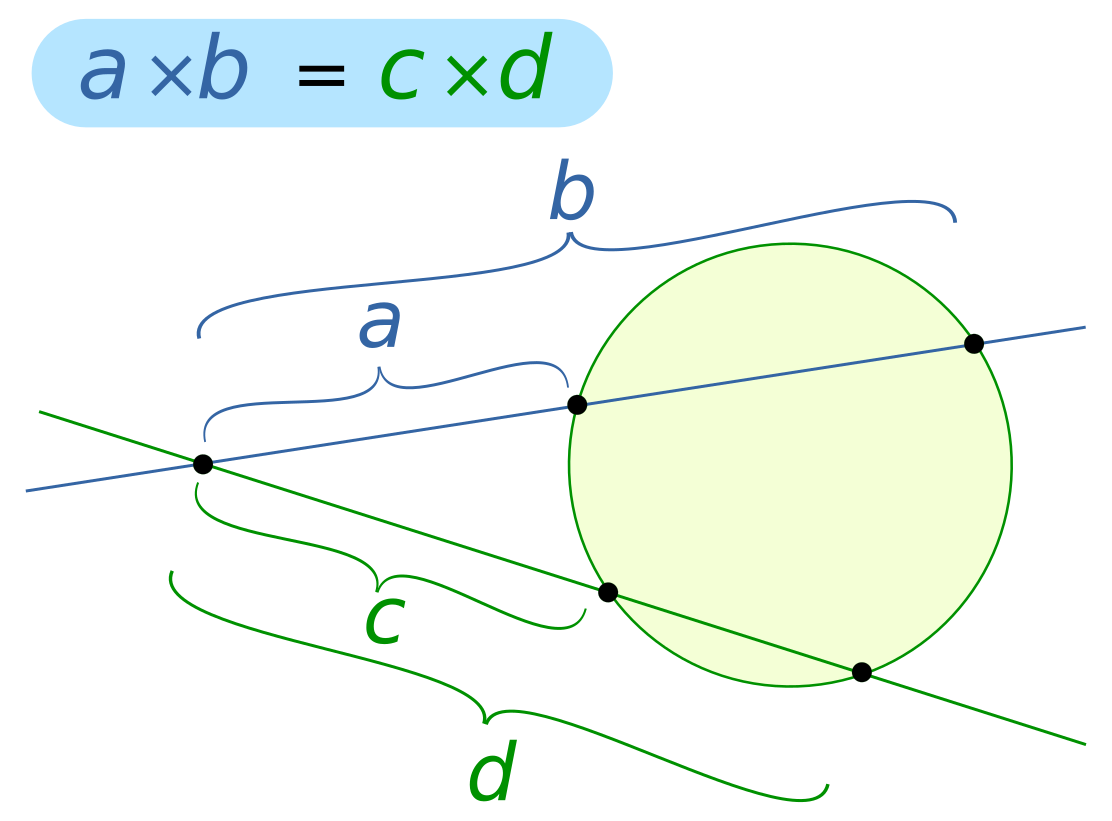
\includegraphics[width=\columnwidth]{teoremasecantes}
\end{center}
\textbf{Teorema de Secante-Tangente}\\
\begin{center}
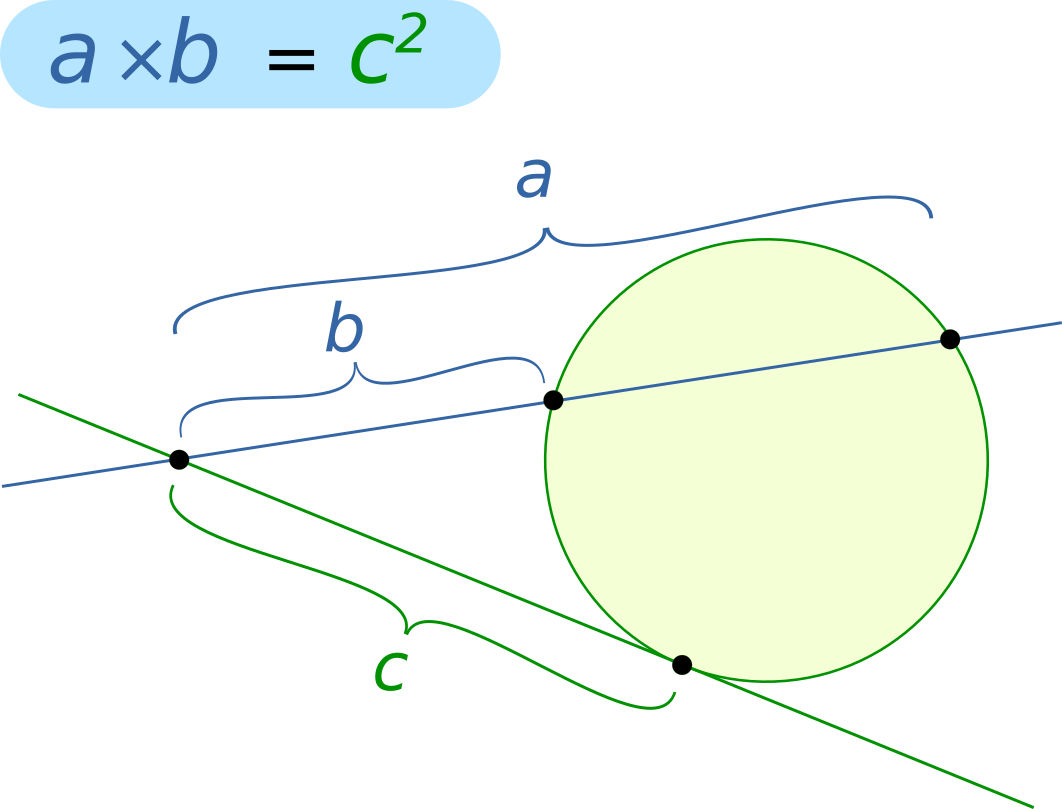
\includegraphics[width=\columnwidth]{teoremasecantetangente}
\end{center}